\documentclass[
 aip,
 jmp,
 amsmath,amssymb,
 reprint
]{revtex4-1}

\usepackage[utf8]{inputenc}
\usepackage[T1]{fontenc}
\usepackage[francais]{babel}
\usepackage{graphicx}
\usepackage{float}
\usepackage{listings}
\usepackage[colorlinks = true, 
            urlcolor = blue]{hyperref}
\usepackage{caption}
\usepackage{dcolumn}
\usepackage{bm}
\lstset{columns=flexible}
\lstset{keepspaces=false}
\begin{document}

\title{Comparatif des performances d'une application en fonction des paramètres de compilation utilisés et analyse des performances}

\author{Pierre \textsc{Tassel} sous la direction de Sid \textsc{Touati}}

\date[Date: ]{\today}

\begin{abstract}
L'utilisation d'outils tels que \textit{GProf} et la suite \textit{Parallel Studio XE d'Intel}\copyright \, nous permettent une analyse plus poussée des programmes et ouvrent la voie vers de possibles optimisations.
\end{abstract}

\maketitle

\hypersetup{linkcolor=blue}
\begin{quotation}
Dans le but de nous familiariser avec les outils d'analyse de performances d'Intel et du projet GNU, nous allons analyser un algorithme de type MinMax avec coupe Alpha Bêta\pageref{Fig:alpha_beta} sur l'une des variantes du jeu Awale\pageref{Fig:awale} avec six cases par joueur écrit en C++. Le but étant de déterminer la meilleure façon de compiler ce programme (compilateur et options à utiliser), d'analyser ce programme pour déterminer ce qui ralentit son exécution ainsi que de tenter de l'optimiser par différents moyens.
\end{quotation}

\hypersetup{linkcolor=black}
\tableofcontents

\hypersetup{linkcolor=blue}
\section{Introduction}
\subsection{Programme à analyser}
Le code à analyser étant dépendant de Windows (import de la bibliothèque windows.h), il faut tout d'abord le réécrire pour permettre de le rendre non dépendant d'un os en particulier. Cette bibliothèque est utilisée pour les compteurs de temps, il est donc facile de réécrire le programme afin qu'il soit indépendant de l'OS en utilisant les fonctions de la librairie standard.\par
Ce programme utilise un algorithme de type MinMax avec coupes alpha bêta\pageref{Fig:alpha_beta} pour le jeu d'Awalé\pageref{Fig:awale}, le principe d'un algorithme MinMax est de parcourir jusqu'à une certaine profondeur l'arbre des coups possibles à un état donné du jeux et d'attribuer un score à chaque coup possible, il choisira ensuite le coup qui lui est le plus favorable en partant du principe que l'adversaire choisira les meilleurs coups. Les coupes alpha bêta sont une technique permettant d'aller plus profondément dans l'arbre des coups possibles en éliminant certains mauvais coups et évitant ainsi beaucoup d'explorations inutiles.

\begin{figure}[H]
  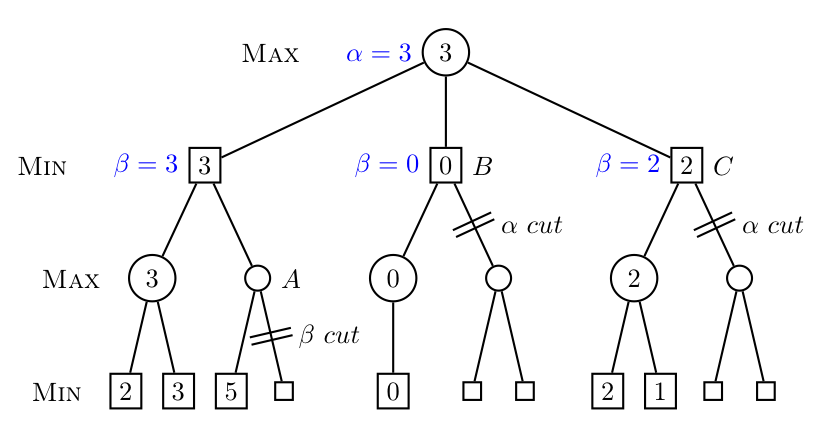
\includegraphics[width=\linewidth, keepaspectratio=true]{alpha_beta.png}
  \centering
  \caption{Algorithme MinMax Alpha-Beta.\label{Fig:alpha_beta}}{\href{https://github.com/LewisMatos/MiniMaxTicTacToe}{Source: Github Lewis Mato.}}
\end{figure}
\begin{figure}[H]
  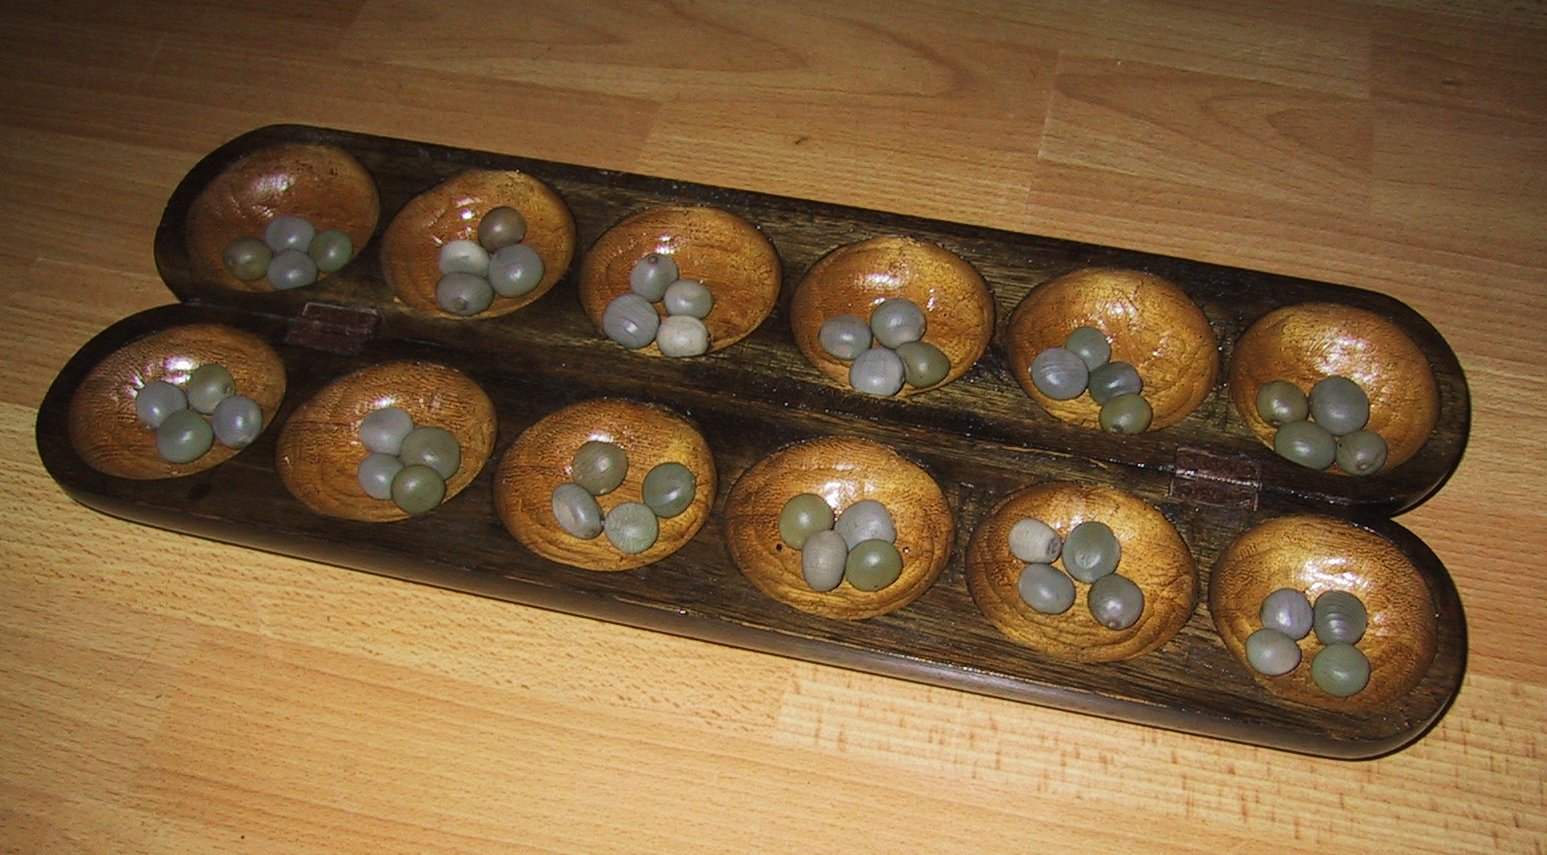
\includegraphics[width=\linewidth, keepaspectratio=true]{Awale.jpg}
  \centering
  \caption{Le jeux de l'Awale.\label{Fig:awale}}{\href{https://fr.wikipedia.org/wiki/Awale}{Source: Wikipedia.}}
\end{figure}

\subsection{Environnement d'analyse}
\subsubsection{Logiciel}
Afin d'analyser le programme efficacement, il faut aussi mettre en place un environnement propice à l'analyse des performances, pour cela nous utiliserons un système d'exploitation en CLI, avec le minimum de services possible installés. Nous utiliserons donc Arch Linux, basé sur le noyau Linux 4.14.13-1 cette distribution possède le minimum d'applications et de services possibles installés.\par
Nous utiliserons trois compilateurs, GCC, ICC (Intel C++ Compiler) et CLang. La version de GCC installée est la version 5.4.0, la version de CLang est la version 6.0.0-1 et celle de ICC est la version 18.0.2.

\subsubsection{Matériel}
Notre environnement expérimental est composé d'un ordinateur portable utilisant un processeur Intel i7-4710HQ, 8Go de RAM en DDR3, un SSD de 120go où le processeurs scaling a été désactivé dans le BIOS, cela permet de faire tourner le processeur à vitesse constante et ainsi de ne pas fausser les résultats.

\begin{figure}[H]
  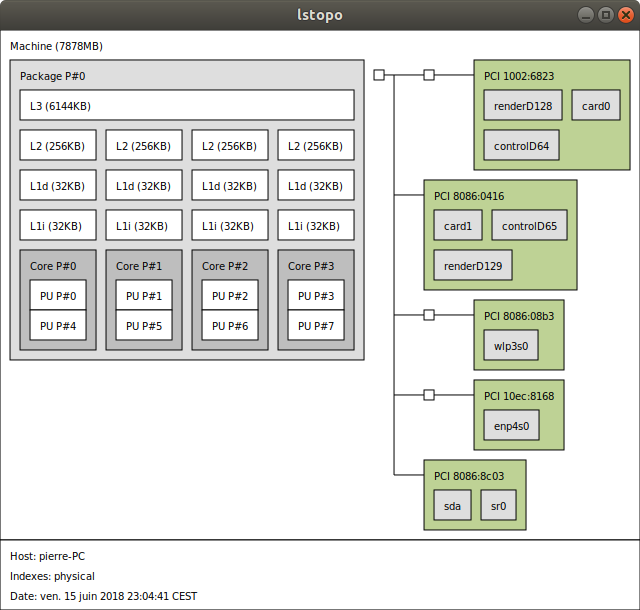
\includegraphics[width=\linewidth, keepaspectratio=true]{caches.png}
  \caption{Topologie des caches de ma machine.\label{Fig:caches}}
\end{figure}

\section{Analyse des options de compilations optimaux}

\subsection{Démarche expérimentale}
Il faut tout d'abord modifier le programme pour qu'il n'affiche en sortie uniquement le temps d'exécution de la partie et non plus les informations utiles aux joueurs.\par
Ensuite, il faut obtenir un ensemble de données. Sachant que le programme est déterministe (pas de modification de la profondeur en fonction du temps, ni de random) les mêmes entrées (coups joués par nous) produiront les mêmes sorties (coups joués par le logiciel). Il nous suffit donc de posséder une liste de coup à envoyer sur la sortie standard des différentes versions du programme (obtenue à partir des différentes options de compilations utilisées) et nous obtiendrons le temps d'exécution de chacun.\par
Afin d'obtenir les entrées du programme, nous avons fait tourner deux instances du programme, l'un jouant le joueur 1, le second jouant le joueur 2 et nous avons noté les coups joués par chacun.\par
A la fin de l'obtention de ces différents coups, nous pouvons déduire que le temps d'exécution sera à analyser en seconde, vu que la partie est plutôt longue.\par
Nous créerons ensuite un script exécutant les différentes compilations et exécuteras les programmes vingt fois chacun pour chaque partie (une fois où le programme commence, une fois où le joueur commence). Cela permettra de déterminer quel est le meilleur compilateur et avec quels options.\par
Ce script étant très lent à s'exécuter (il y a 480 exécutions différentes au total) nous l'exécuterons au travers de la commande \textbf{nohup} afin d'éviter toute interruption possible.

\subsection{Résultats}
En regardant les temps d'exécutions configuration par configuration nous observons que les temps d'exécutions sont plutôt stables. Nous choisissons donc d'afficher les résultats sous forme de barres représentant la médiane des temps d'exécutions de chaque configuration.

\begin{figure}[H]
  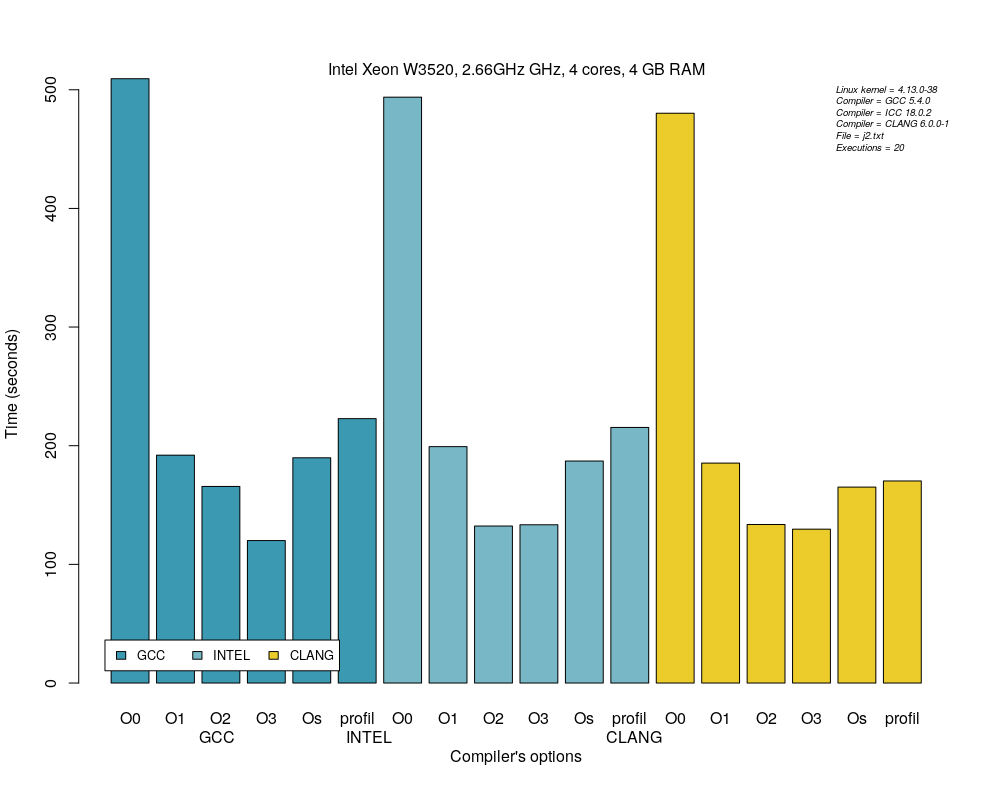
\includegraphics[width=\linewidth, keepaspectratio=true]{GCCvsICCvsCLANG_j2.png}
  \caption{Temps d'exécutions quand le programme commence.\label{Fig:temps_exec_j2}}
  \end{figure}
\begin{figure}[H]
  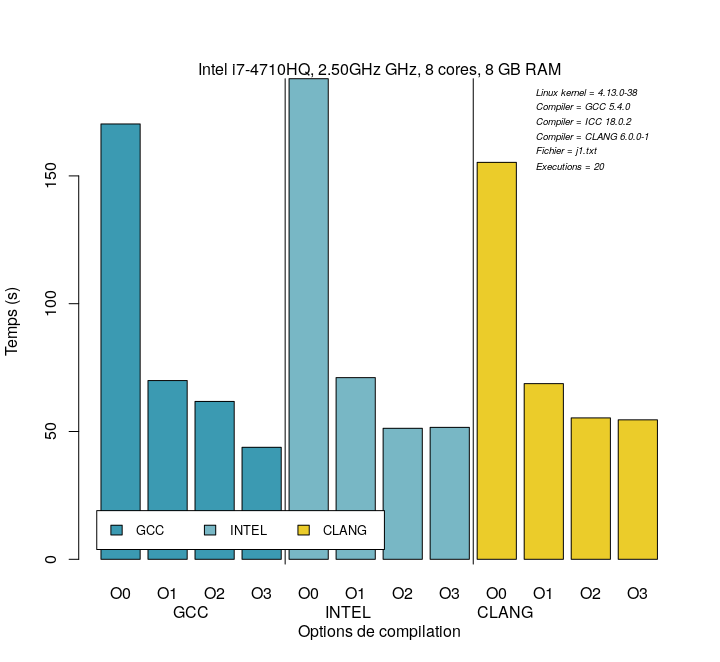
\includegraphics[width=\linewidth, keepaspectratio=true]{GCCvsICCvsCLANG_j1.png}
  \caption{Temps d'exécutions quand le joueur commence.\label{Fig:temps_exec_j1}}
\end{figure}

On remarque que le fait que le joueur commence\pageref{Fig:temps_exec_j1} ou non\pageref{Fig:temps_exec_j2} n'a pas d'influence sur le choix du compilateur, on pourra donc se concentrer sur l'analyse des temps d'exécutions quand le programme commence.\par
On remarque aussi que GCC avec l'option \textbf{O3} activée est le meilleur compilateur pour ce programme.\par
Pour GCC et Intel, chaque niveau d'optimisation réduit grandement le temps d'exécution, il y a un rapport de quatre entre la compilation sans optimisation (\textbf{O0}) et la compilation avec le plus d'optimisations (\textbf{O3}). Cette différence est légèrement inférieure avec CLang, car la version sans optimisation (\textbf{O0}) est plus rapide que celle des autres compilateurs, mais elle reste d'un facteur trois.\par
Une chose étonnante est que la version \textbf{O2} d'Intel est légèrement plus rapide que la version \textbf{O3}.

\subsubsection{Taille des exécutables}
\begin{figure}[H]
  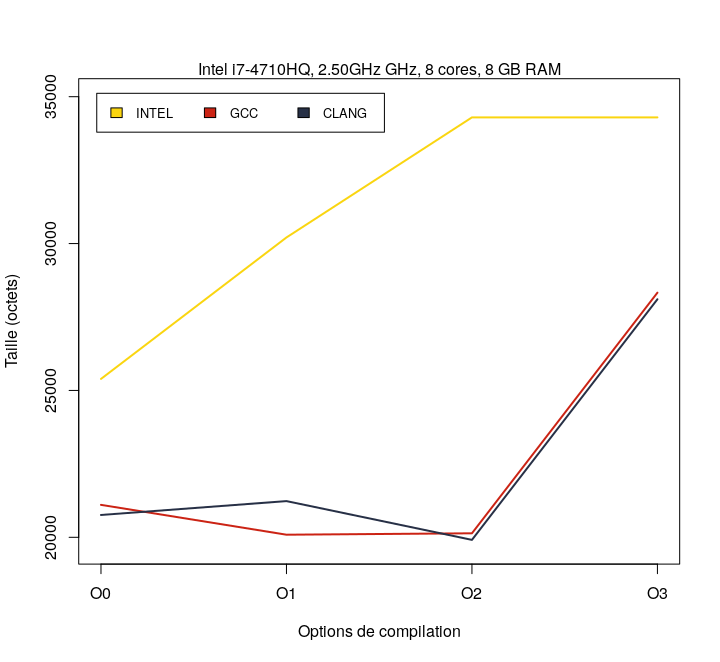
\includegraphics[width=\linewidth, keepaspectratio=true]{tailles.png}
  \caption{Comparatif des tailles d'exécutables produits par diverses méthodes de compilations.\label{Fig:taille_executables_seq}}
\end{figure}

GCC avec l'option \textbf{O3} semble être, là aussi, la meilleure option pour ce programme.

\section{Profilage du code}

Il existe deux grands logiciels pour analyser les performances d'un programme et les fonctions chaudes, GProf qui est un logiciel libre et vTune qui est un logiciel propriétaire appartenant à Intel. Nous allons utiliser ces deux logiciels, afin de trouver des possibilités d'optimisation de code.

\subsection{Gprof}

\begin{figure}[H]
  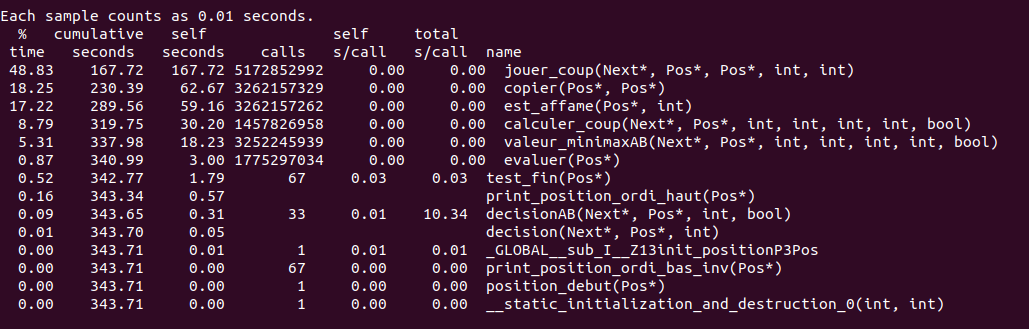
\includegraphics[width=\linewidth, keepaspectratio=true]{gprof1.png}
  \caption{Fonctions chaudes d'après GProf.\label{Fig:gprof_flat}}
\end{figure}

Il nous apprend que la fonction la plus utilisée est \textbf{\textit{jouer\_coup}}, et ce très largement, cependant on remarque qu'il y a énormément d'appel (plus de cinq milliards) mais que chaque appel est extrêmement rapide. On note aussi que la fonction \textbf{decisionAB} est moins souvent appelée, mais chaque appel est d'une plus longue durée (dix secondes par appel en moyenne).\par
Ce sont donc les deux fonctions qu'il faut tenter d'optimiser en priorité pour améliorer les performances d'après GProf.

\subsection{Intel vTune}

\begin{figure}[H]
  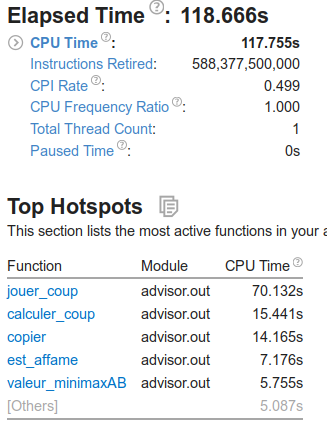
\includegraphics[width=\linewidth, keepaspectratio=true]{vtune.png}
  \caption{Profilage du code avec vTune.\label{Fig:vTune_sequentiel_cpu}}
\end{figure}

Comme GProf, vTune nous indique que c'est la fonction \textbf{jouer\_coup} qui a pris le plus de temps à calculer. Cependant, il place \textbf{calculer\_coup} second contrairement a GProf.\par
Il nous apprend aussi que seul un processeur est utilisé sur les huits disponibles. Il y a donc un manque de parallélisme, ce qui ouvre une première voie vers une possible optimisation.\par
Nous pouvons aussi utiliser ce logiciel pour analyser les accès mémoire.

\begin{figure}[H]
  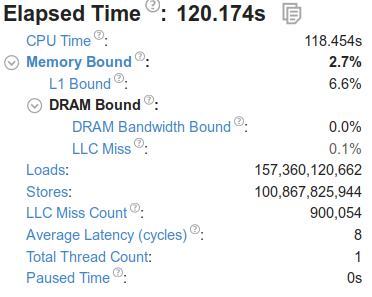
\includegraphics[width=\linewidth, keepaspectratio=true]{memory_vtune.png}
  \caption{Profilage des accès mémoire.\label{Fig:vTune_sequentiel_mem}}
\end{figure}

On remarque très clairement que le programme n'est pas "Memory Bottleneck" mais "CPU Bottleneck" (le CPU est le facteur limitant de cette application).\par
Car il y a très peu d'erreurs de cache et les accès mémoire sont petits et rapides.

\section{Ajout de parallélisme}

Comme ce programme est CPU Bottleneck et qu'il n'y a qu'un seul processeur utilisé, l'ajout de parallélisme semble être une possibilité d'optimisation.

\subsection{Approche naïve}

\subsubsection{Démarche expérimentale}

On a ajouté du parallélisme un peu partout où il n'y a pas de dépendance de données en utilisant la librairie OpenMP.\par
Malheureusement, il a été impossible de rajouter du parallélisme de contrôle, mais seulement du parallélisme de données, on peut d'ores et déjà s'attendre à ce que le parallélisme soit peu pertinent vu la faible taille des données et la simplicité des actions effectuées dans chacune des itérations des boucles parallélisées.\par
Ensuite, nous réitérons ce que nous avons fait pour la version sans parallélisme en utilisant chaque compilateur avec l'option \textbf{O3} activé mais, en faisant varier le nombre de processeurs pour déterminer le nombre optimal de processeur à utiliser.

\subsubsection{Résultats}

Nous représentons les résultats sous forme de \href{https://en.wikipedia.org/wiki/Violin_plot}{Violin Plot} nous permettants de représenter à la fois les écarts types et la fonction de densité.

\begin{figure}[H]
  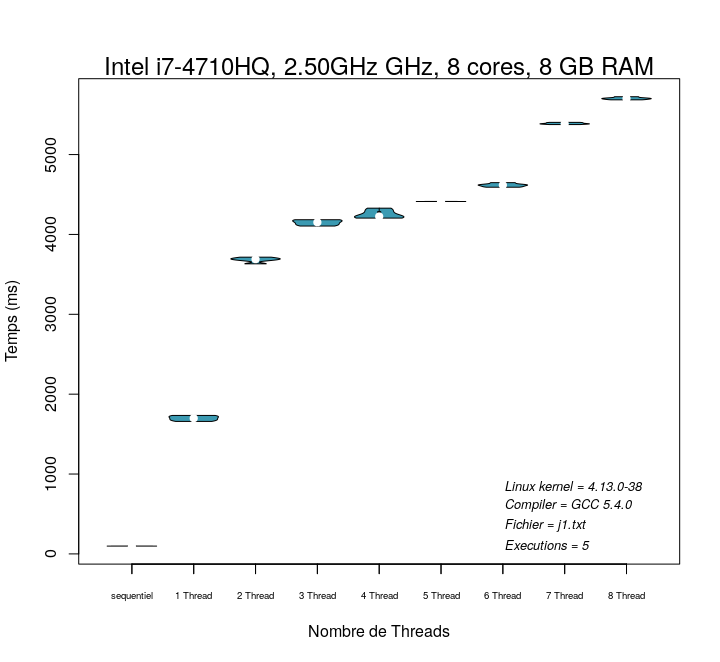
\includegraphics[width=\linewidth, keepaspectratio=true]{gcc_parallel_naif.png}
  \caption{Résultat ajout parallélisme de façon naïve avec GCC.\label{Fig:gcc_naif}}
\end{figure}

\begin{figure}[H]
  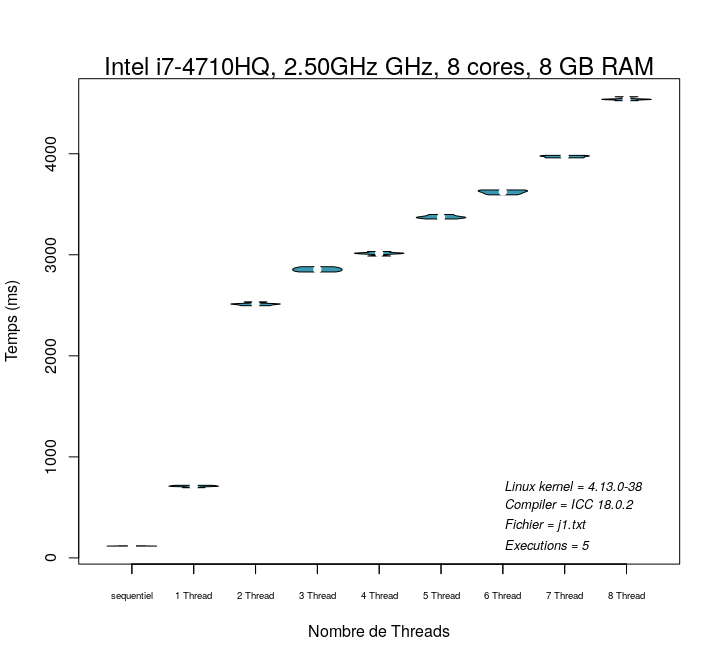
\includegraphics[width=\linewidth, keepaspectratio=true]{intel_parallel_naif.png}
  \caption{Résultat ajout parallélisme de façon naïve avec Intel.\label{Fig:intel_naif}}
\end{figure}

\begin{figure}[H]
  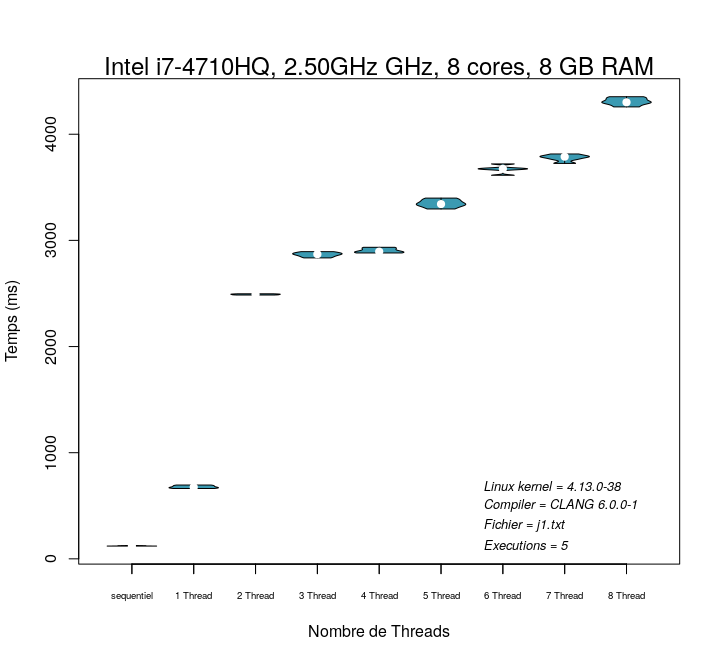
\includegraphics[width=\linewidth, keepaspectratio=true]{clang_parallel_naif.png}
  \caption{Résultat ajout parallélisme de façon naïve avec CLang.\label{Fig:clang_naif}}
\end{figure}

Nous devons malheureusement réduire le nombre d'exécutions par configuration passant de vingt à cinq, car le temps d'exécutions est extrêmement lent.\par
On remarque ici que CLang\pageref{Fig:clang_naif} et Intel\pageref{Fig:intel_naif} sont côte à côte niveau performance et qu'ici GCC\pageref{Fig:gcc_naif} pourtant le plus rapide sur le code séquentiel est le plus lent avec la version parallèle.\par
On remarque aussi que le temps d'exécutions c'est nettement dégradé quel que soit le compilateur utilisé et qu'il se détériore de plus en plus quand on ajoute un plus grand nombre de processeurs. Cela est probablement dû à deux facteurs : 
\begin{enumerate}
\item Le phénomène de False Sharing\pageref{Fig:false_sharing}, les différents processeurs doivent assurer la cohérence des caches, à chaque fois qu'un processeur modifie une donnée, il invalide le cache d'un autre processeur s'il modifie la même ligne cache. Ce qui explique pourquoi augmenter le nombre de threads n'améliore pas les performances du programme, mais au contraire le ralentit encore plus.
\item OpenMP casse les optimisations du compilateur en ajoutant du code qui va aveugler le compilateur. Cela explique pourquoi les performances sont nettement inférieure entre le code séquentiel et le code avec un seul thread.
\end{enumerate}

\begin{figure}[H]
  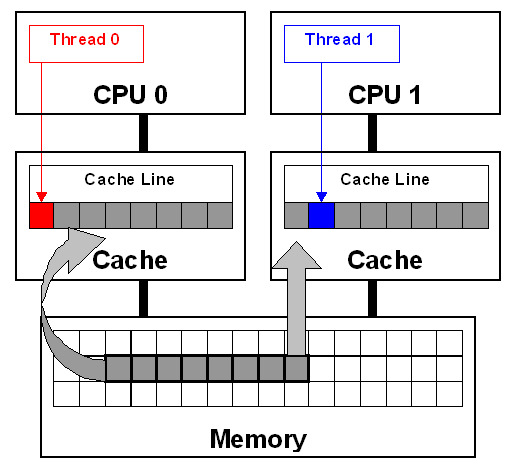
\includegraphics[width=\linewidth, keepaspectratio=true]{false_sharing.jpg}
  \centering
  \caption{Mécanisme de False Sharing.\label{Fig:false_sharing}}{\href{https://software.intel.com/en-us/articles/avoiding-and-identifying-false-sharing-among-threads}{Source : Documentation Intel.}}
\end{figure}

Pour confirmer notre hypothèse, nous pouvons utiliser le logiciel vTune afin d'analyser cette version parallélisée avec huit threads.\par
A cause de la limitation de 500MB de collection de données par analyse, le programme s'arrête avant la fin, mais sachant que le programme est constitué d'une boucle principale qui se répète jusqu'à la fin de la partie, les données collectées restent pertinente et représentative de l'ensemble du programme.

\begin{figure}[H]
  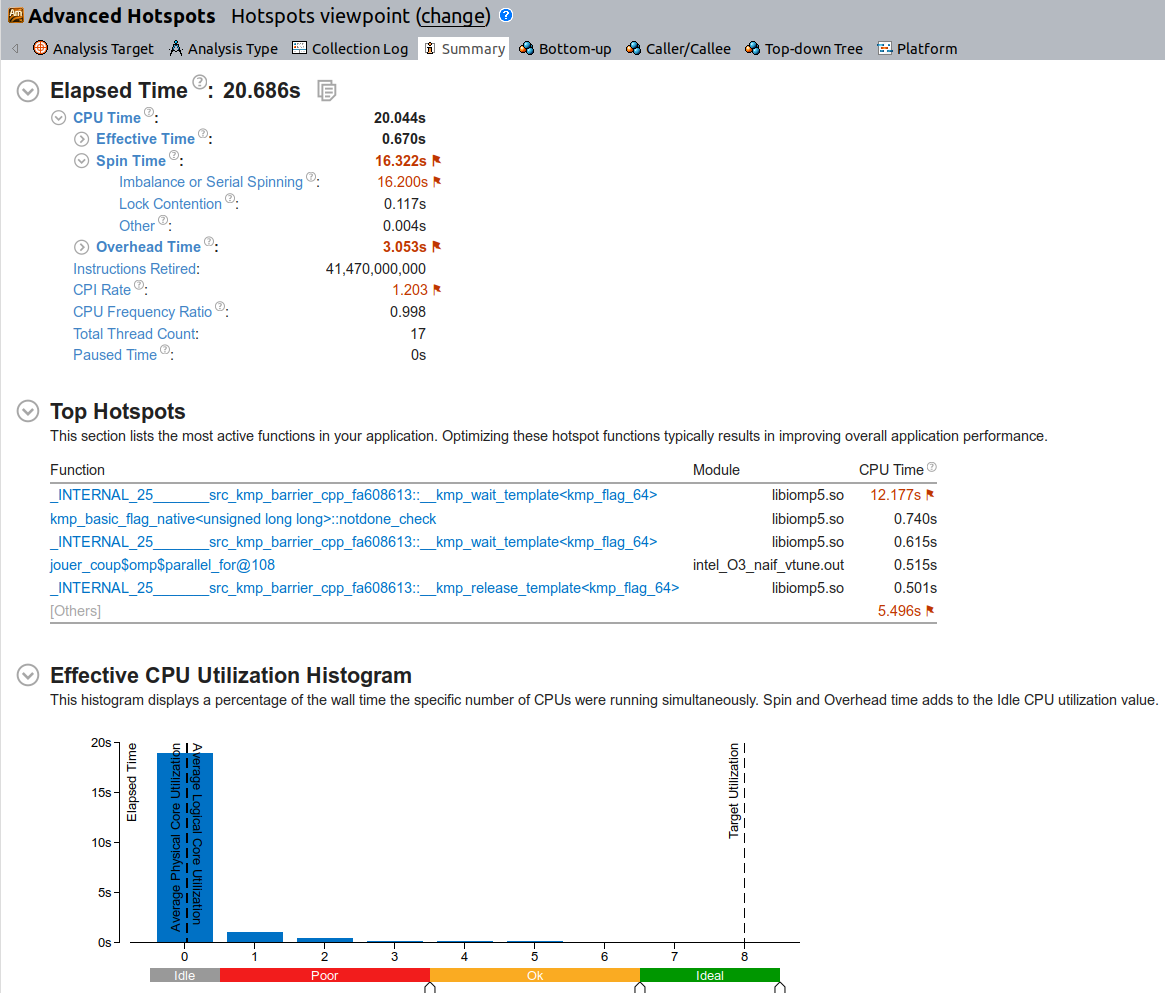
\includegraphics[width=\linewidth, keepaspectratio=true]{vtune_parallel.png}
  \centering
  \caption{vTune version parallèle\label{Fig:vtune_proc_use}}
\end{figure}

On remarque que le CPU passe beaucoup de temps à attendre la fin de chaque thread (Spin time) seize secondes sur les vingt secondes d'exécutions et beaucoup de perte de temps en création des threads et en temps de placement de ces threads (3 secondes sur 20). Le temps de calcul effectif n'est que de 0.6 secondes sur 20, ce qui confirme la non-pertinence du parallélisme tel qu'il a été ajouté.

\begin{figure}[H]
  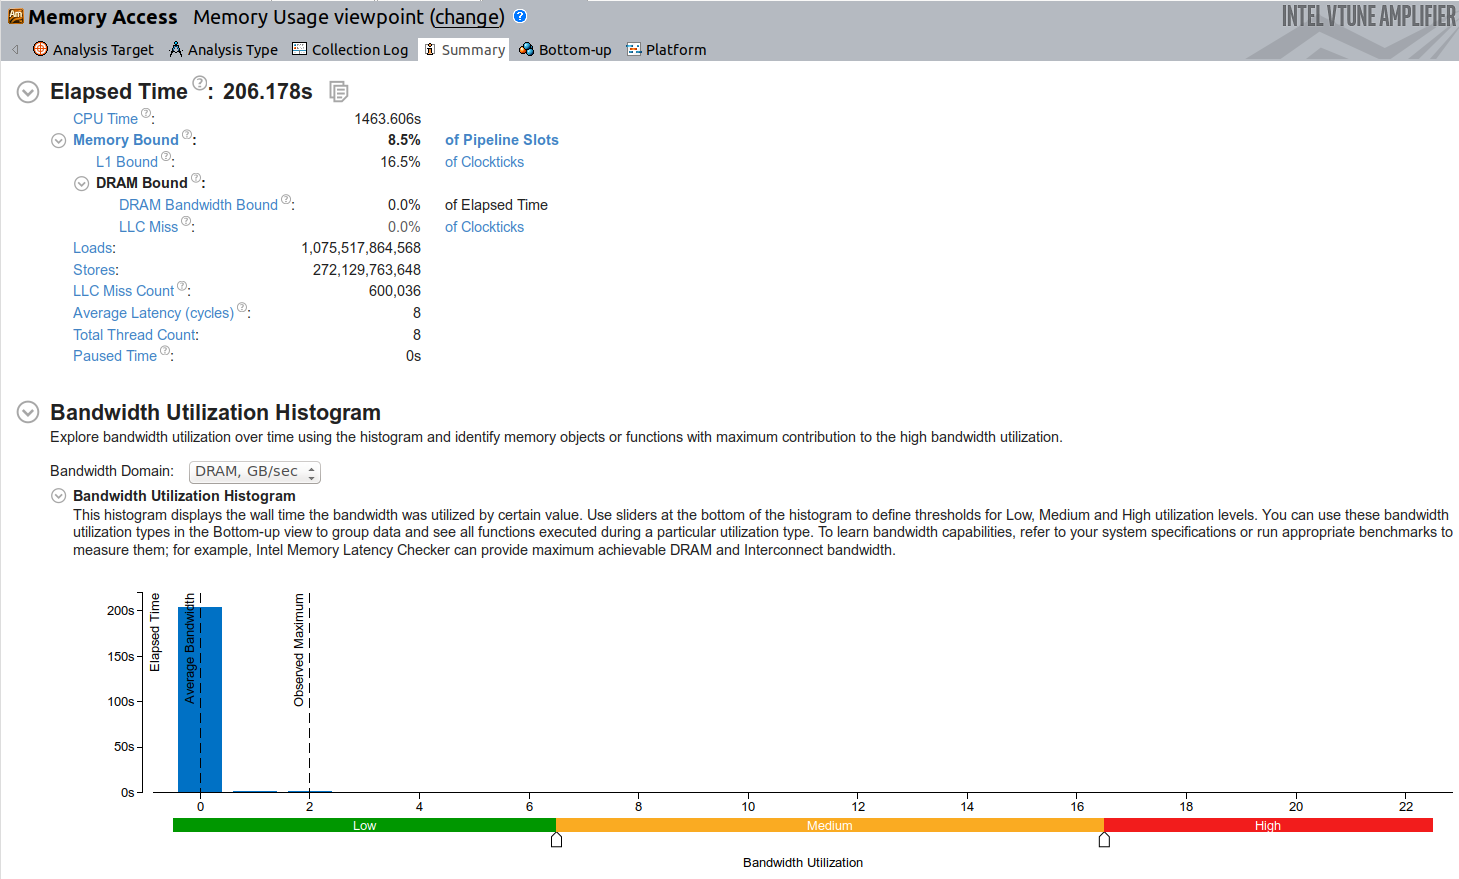
\includegraphics[width=\linewidth, keepaspectratio=true]{vtune_parallel_memory.png}
  \centering
  \caption{vTune version parallèle avec analyse de la mémoire.\label{Fig:vtune_mem_use}}
\end{figure}

L'analyse de mémoire confirme le False Sharing\pageref{Fig:false_sharing}, en effet il y a 16.5\% de "L1 Bound" (défaut de cache L1) qui ont sûrement été causé par le mécanisme de False Sharing expliqué précédemment.

\subsection{Tentative d'amélioration des performances du code parallèle en modifiant le placement des threads}

Un facteur qui peut être important dans les performances des codes parallèles est la manière dont sont placés les threads, cette méthode de placement de thread est appelée le "thread affinity".

\begin{figure}[H]
  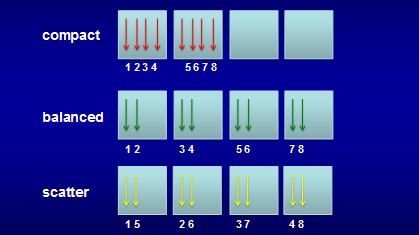
\includegraphics[width=\linewidth, keepaspectratio=true]{affinity.png}
  \centering
  \caption{Différentes méthodes de placement de thread. \label{Fig:affinity}}{\href{https://cvw.cac.cornell.edu/mic/affinity}{Cornell University}}
\end{figure}

Nous allons voir si modifier le placement des threads améliore ou non les performances parallèles en utilisant le compilateur d'Intel avec huit threads car c'est l'un des compilateurs qui offrait les meilleures performances parallèle et il a une gestion du placement des threads plus complète que Clang. Nous testerons deux méthodes de placement "Compact" et "Scatter"\pageref{Fig:affinity} supporté par le compilateur Intel en utilisant la variable d'environnement \href{https://software.intel.com/en-us/node/522691}{KMP\_AFFINITY}.

\begin{figure}[H]
  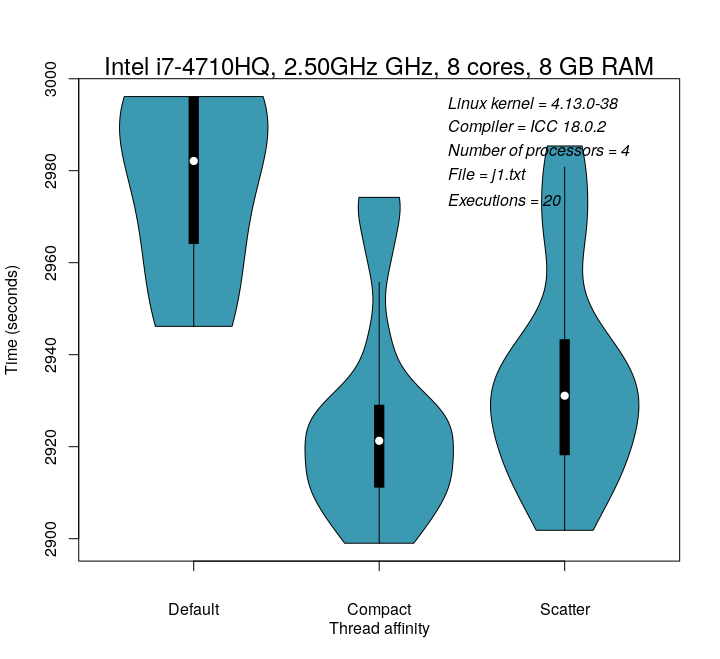
\includegraphics[width=\linewidth, keepaspectratio=true]{defaultVSscatterVScompact.png}
  \caption{Comparaison performances Scatter vs Compact.\label{Fig:scatter_vs_compact}}
\end{figure}

On remarque que les performances se sont bien améliorées par rapport au mode de placement par défaut (celle de l'OS lui-même). Les performances de Compact et Scatter sont à peu près équivalentes\pageref{Fig:scatter_vs_compact} pour ce programme-ci dans cette configuration.

\subsection{Intel Advisor}

Advisor est un autre logiciel de la suite Parallel Studio qui, en plus de nous informer sur les fonctions chaudes du programme, nous donne des indications sur comment optimiser le code.\par
Nous avons vu que l'ajout naïf de parallélisme était défavorable aux performances du programme, nous allons ici tenter d'ajouter du parallélisme de manière plus intelligent à l'aide des outils de la suite Intel Parallel Studio XE.

\begin{figure}[H]
  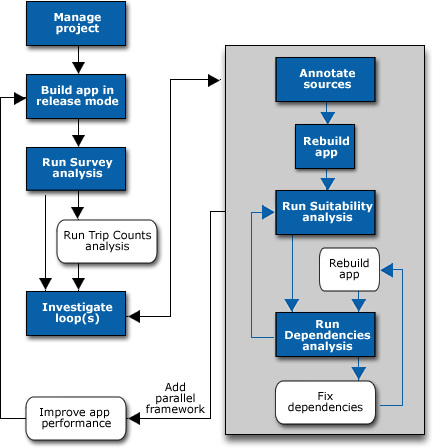
\includegraphics[width=\linewidth, keepaspectratio=true]{Intel.jpg}
  \centering
  \caption{Processus itératif d'amélioration des performances.\label{Fig:intel_processes}}{\href{https://software.intel.com/en-us/node/684712}{Source : Documentation Intel.}}
\end{figure}

\paragraph{Fonctions chaudes et optimisations}
D'abord, nous analysons le programme en cherchant les fonctions chaudes et les différents problèmes pouvant réduire les performances du programme.

\begin{figure}[H]
  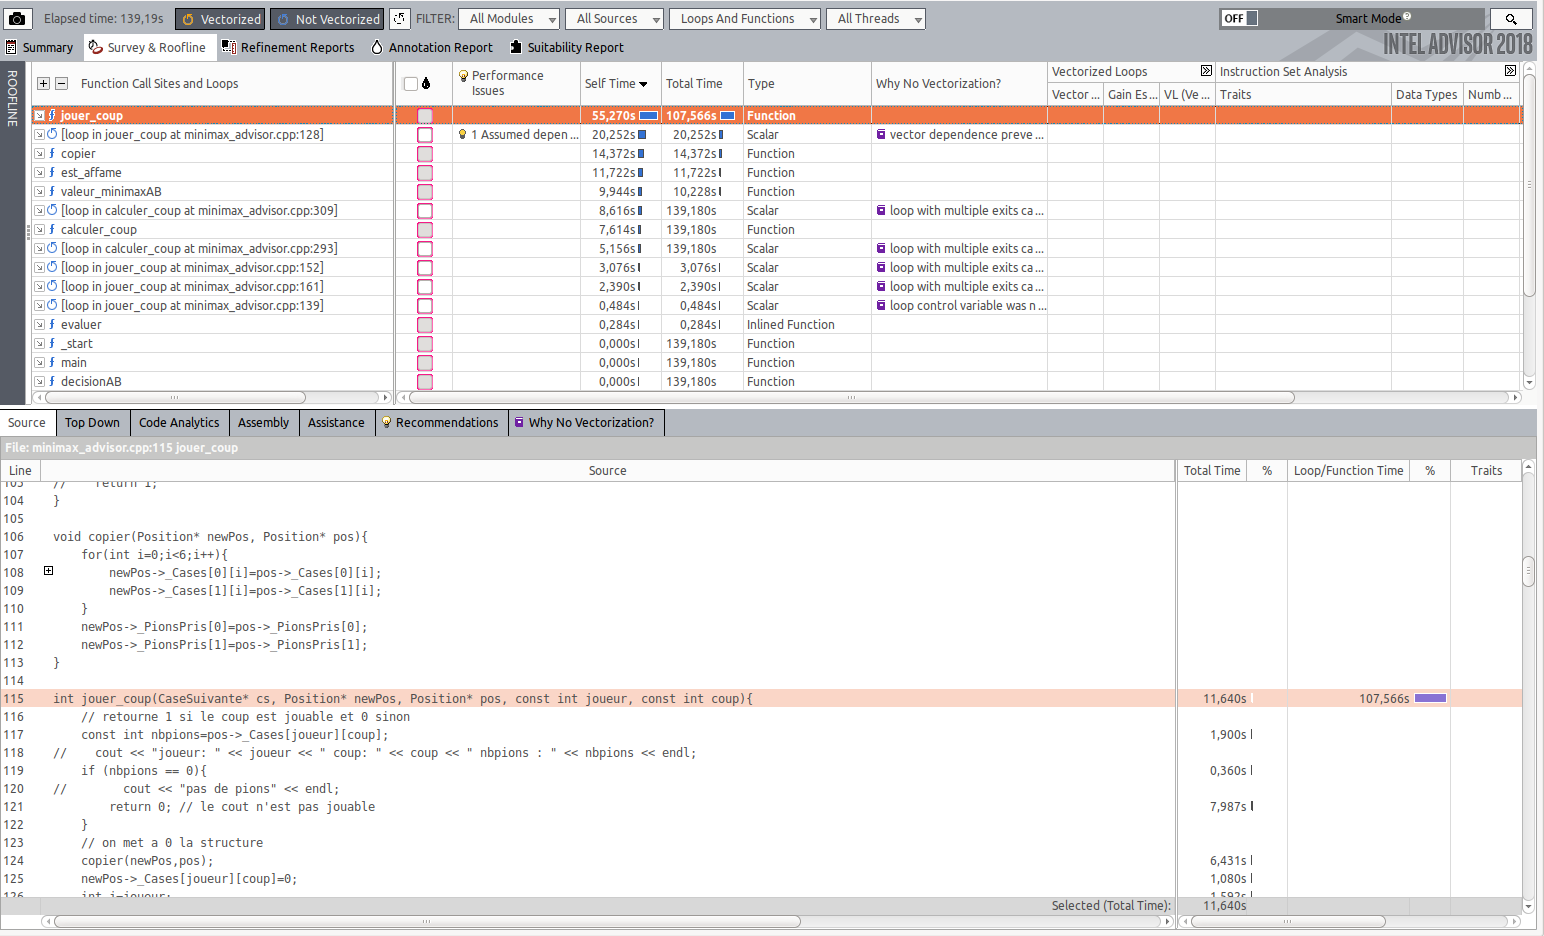
\includegraphics[width=\linewidth, keepaspectratio=true]{survey.png}
  \caption{Résultat d'Advisor "Survey".\label{Fig:advisor_survey}}
\end{figure}

Contrairement à vTune\pageref{Fig:vtune_proc_use}, Advisor donne aussi des indications sur ce qui nuit aux performances du programme. Par exemple nous avons ici une dépendance de donnée qui empêche la vectorisation. Malheureusement nous ne pouvons pas la supprimer, car c'est une dépendance Read after Write (dite "true dependancy").

\subsubsection{Test opportunité ajout de parallélisme}

Il faut donc chercher où il convient d'ajouter du parallélisme afin que cela augmente les performances du programme.\par
Pour cela nous visons les boucles ou le programme passe plus de 1.5\% du temps afin que l'ajout de parallélisme soit un minimum pertinent, idéalement on choisirait les boucles où l'on passe au moins 5\% du temps, mais il n'y en a aucune dans ce programme, car il effectue beaucoup d'appel récursif.\par
Nous ajoutons des annotations autour des zones que nous souhaiterions idéalement paralléliser et nous exécutons une analyse dite de "Suitability".

\begin{figure}[H]
  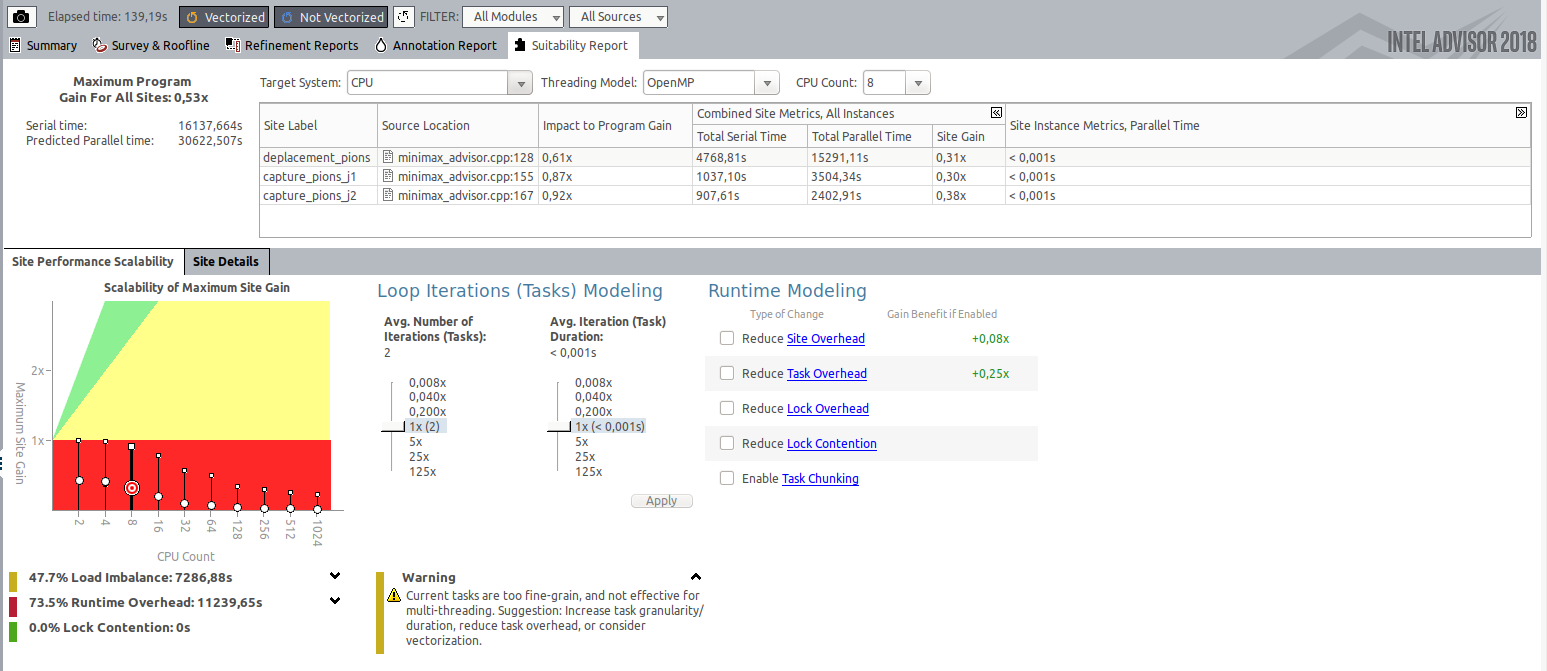
\includegraphics[width=\linewidth, keepaspectratio=true]{suitability.png}
  \caption{Résultat d'Advisor "Suitability".\label{Fig:advisor_suitability}}
\end{figure}

Malheureusement nous pouvons observer que l'ajout de parallélisme à chaque boucle ne fera que ralentir le programme.\par
Le logiciel nous indique que les taches effectuées sont d'une granularitée trop fine ce qui induit un "Task Overhead" (le temps passé à créer une tâche et à l'assigner à un thread ainsi qu'à mettre en pause ou arrêter le thread une fois fini) qui est trop important, ce qui pénalise le programme parallèle.

\subsubsection{Test de la viabilitée ajout parallélisme}

Malgré le fait que l'ajout de parallélisme ne soit pas pertinent, nous allons tout de même tester le mode "Dependencies" d'Advisor qui sert à détecter si les hotspots dont l'ajout de parallélisme est pertinent découvert précédemment ne possèdent pas des dépendances de données qui empêchent la parallélisation.

\begin{figure}[H]
  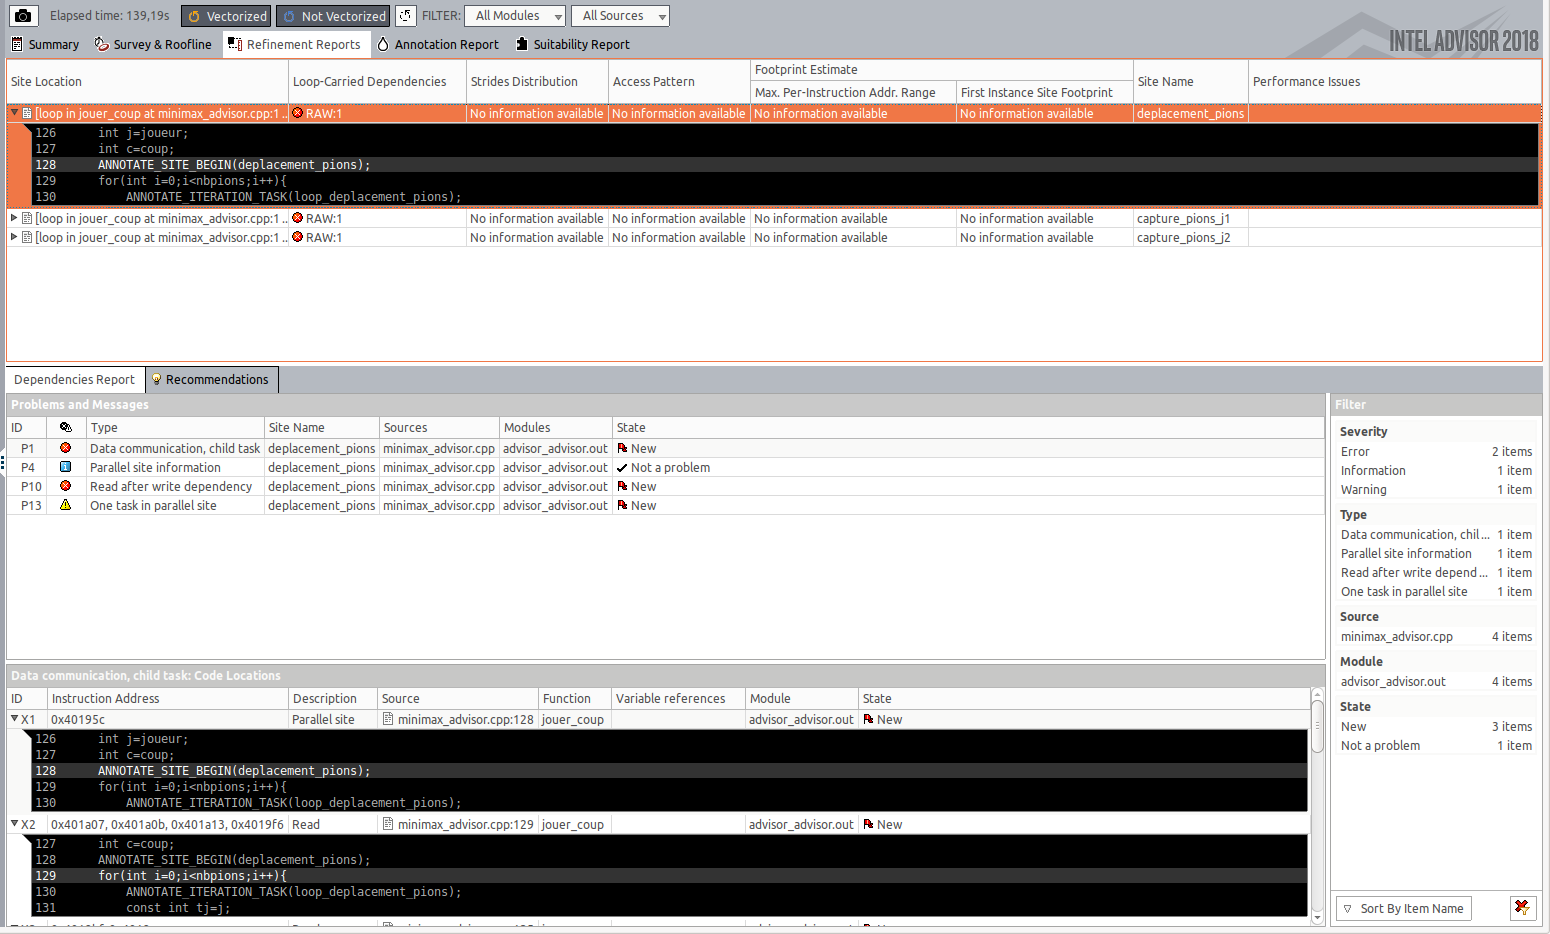
\includegraphics[width=\linewidth, keepaspectratio=true]{dependecies.png}
  \caption{Résultat d'Advisor "Dependencies".\label{Fig:advisor_dependencies}}
\end{figure}

En plus de ne pas être pertinent, l'ajout de parallélisme dans les hotspots n'est pas possible à cause des dépendances de données, Read After Write donc réelles dépendances que l'on ne peut enlever. Et il n'est pas non plus possible d'ajouter du parallélisme dans la fonction \textbf{decisionAB} à cause du fait qu'il faille remonter alpha et bêta\pageref{Fig:alpha_beta} lors de l'évaluation des sous-noeuds afin d'effectuer des coupes.

\section{Modification algorithmique du code}

Dans cette partie nous allons essayer d'améliorer les performances de notre application en modifiant son algorithme.\par
Ce programme utilise un algorithme de min-max avec coupes alpha bêta\pageref{Fig:alpha_beta}, il y a quelques voies d'optimisation possible :
\begin{enumerate}
\item Nous pourrions réordonner l'ordre d'évaluation des coups afin de faire jouer les coups statistiquement meilleurs en premier (exemple: un puits avec beaucoup de cailloux à plus de chance d'être un meilleur coup qu'un puits avec un unique cailloux). Cela peut améliorer l'efficacité des coupes alpha bêta\pageref{Fig:alpha_beta}.
\item Nous pourrions créer une table de transposition qui associe une position à un score afin de ne pas avoir à recalculer certaines positions. Vu que l'on doit utiliser une fonction de hachage, il y a potentiellement des collisions qui peuvent changer les coups joués par rapport à la version sans table de transposition, mais il est très facile de tester si tel est le cas.
\item On peut créer un fichier d'ouvertures, avec les X premiers coups pré-calculés à l'avance avec une meilleure profondeur. L'inconvénient de cette solution est qu'elle peut changer les coups joués par la nouvelle version du programme par rapport à la version de base, ce qui empêche la comparaison.
\end{enumerate}

\subsection{Trie des coups à visiter}
Trier à chaque profondeur à un coup trop important, mais trier à la profondeur zéro est pertinent, car cela peut aider grandement à améliorer la valeur de alpha\pageref{Fig:alpha_beta} et donc de générer plus de coupe dans les sous noeuds, et ce pour un coût négligeable en temps (trie sur les indices d'un tableau de six cases).

\begin{figure}[H]
  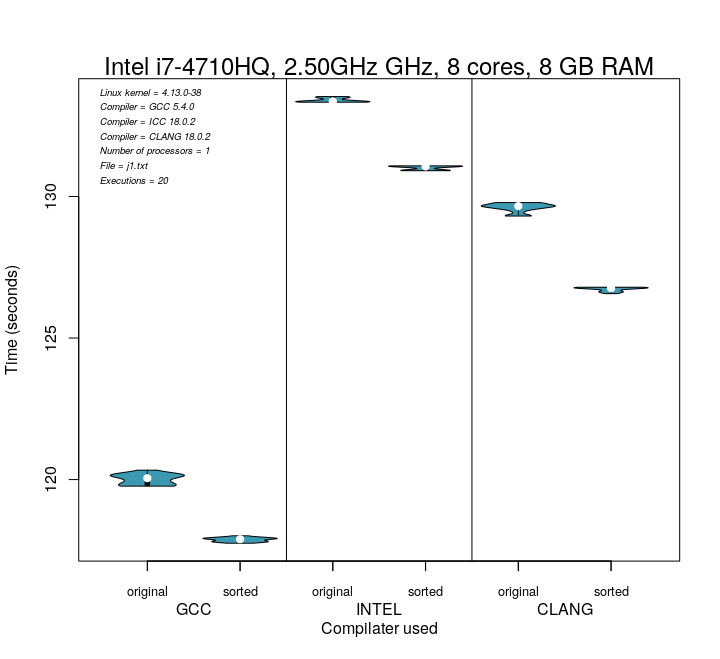
\includegraphics[width=\linewidth, keepaspectratio=true]{trie.png}
  \caption{Trie coup au premier niveau.\label{Fig:trie_coup}}
\end{figure}

On remarque qu'il y a eu une amélioration des performances assez nette, d'environ 30\%. C'est donc une optimisation à garder.

\subsection{Table de transposition}
On ne peut pas avoir une table de hashage globale car il y a trop de positions possibles à stocker. Cependant, on peut avoir une table de hashage pour le tour courant, qui nous permet de regarder pour chaque noeud, si il a déjà été évalué et cela peut, peut-être nous éviter certains calculs sans pour autant consommer trop de mémoire.

\subsubsection{Ordered Map}
En C++ les \textbf{std::map} sont des arbres binaires de recherche. Pour pouvoir implémenter les maps il faut d'abord changer légèrement la structure de données contenant la position du plateau, passant d'un tableau deux dimensions à un objet de type \textbf{std::array} à une dimension (on linéarise simplement le tableau à deux dimensions).

\begin{figure}[H]
  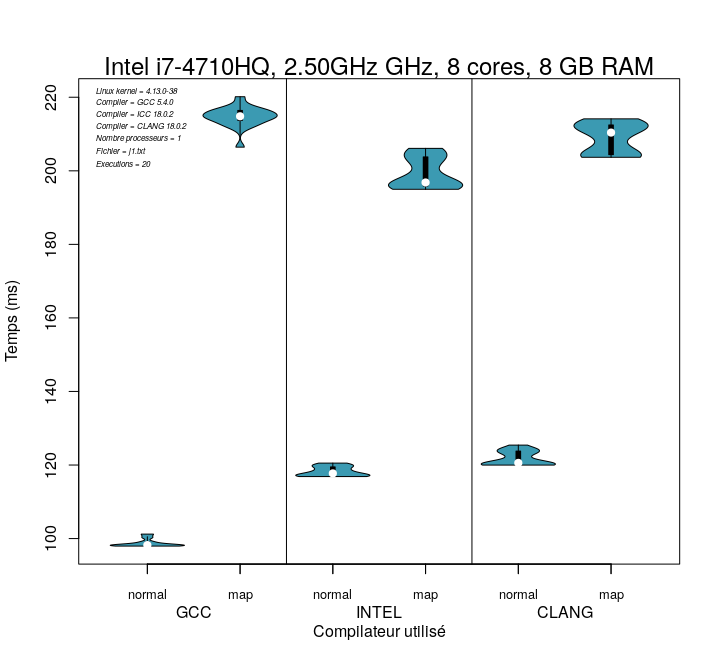
\includegraphics[width=\linewidth, keepaspectratio=true]{sorted_map.png}
  \caption{Ordered Map.\label{Fig:ordered_map}}
\end{figure}

\subsubsection{Unordered Map}
Nous utilisons une fonction de hachage basique trouvé sur \href{https://stackoverflow.com/a/42701911}{StackOverflow}, c'est une fonction qui comme beaucoup de fonction de hashage est basé sur des XOR successifs. Elle effectue des XOR entre le hash de chacun des éléments du tableau auquel on ajoute un nombre fixe, l'élément décalé de six bits vers la gauche et de deux bits vers la droite.

\begin{figure}[H]
  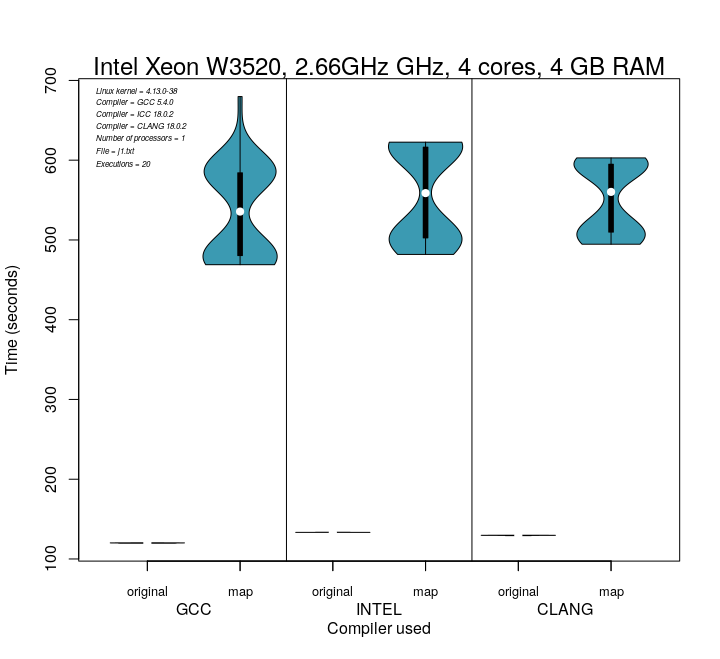
\includegraphics[width=\linewidth, keepaspectratio=true]{unsorted_map.png}
  \caption{Unordered Map.\label{Fig:unsorted_map}}
\end{figure}

Dans les deux cas les performances ne sont pas améliorés, cependant la table de hashage ordonnée donne de meilleurs résultats que la table de hashage non ordonnée, cela semble montrer que la fonction de hashage prend beaucoup de temps à être calculée par rapport au coût de notre fonction d'évaluation (simple différence entre le nombre de cailloux prix par l'ordinateur et l'adversaire).\par
Il est aussi possible que la fonction de hashage ainsi que la structure de donné ne soit pas optimale pour ce jeu, une possibilité serait d'implémenter la \href{https://chessprogramming.wikispaces.com/Zobrist+Hashing}{fonction de hashage de Zobrist} et d'utiliser un grand tableau de liste contenant un couple <Hash,Valeur>, pour retrouver la valeur de notre position, il faudrait faire \textbf{Hash\%TAILLE\_TABLEAU} pour obtenir l'indice du tableau et parcourir jusqu'à trouver notre couple \textbf{<Hash,Valeur>}, si le tableau est très grand cela pourrait peut-être accélérer le calcul, cela n'a pas été fait par manque de temps. Néanmoins, il est fort probable que l'ajout d'une table de hashage soit beaucoup moins pertinent que pour des jeux tel que les échecs, car il y a beaucoup moins de positions répétitives que les échecs.\par
Aux échecs excepté les pions, les pièces peuvent revenir au coup d'après sur leur case d'origine si elles n'ont pas été capturées, si la voix n'est pas bloquée ou si elle ne met pas en échec le roi.

\section{Gestion du projet}
Je me suis servi de \href{https://github.com/ingambe/ter/}{Github} pour héberger mon projet. Je me suis servi de mon ordinateur portable car malheureusement il fallait désactiver le processeur scaling pour éviter de fausser les résultats et cela nécessitait un accès au BIOS, ce qui n'était pas possible avec les serveurs de l'INRIA.\par
Cela était parfois contraignant, car certains programmes ont tourné quasiment quatre jours, mais aussi parce que la distribution installée étant en CLI, je ne pouvais pas l'installer sur mon disque dur principal (car inutilisable pour des tâches quotidiennes), j'ai donc du l'installer sur un autre SSD et changer les disques quand je devais lancer l'expérience.\par
Les résultats ont été obtenus en utilisant des scripts que j'ai écrits en bash, toujours lancé avec la commande nohup (afin d'éviter les interruptions systèmes) et  env -i afin d'éviter d'ajouter des variables d'environnements non propre au script qui viendrait possiblement polluer l'expérience, excepté pour le script de compilation qui a besoin de variables d'environnement pour faire fonctionner le compilateur d'Intel.\par
Les courbes ont été tracées avec le langage R et le rapport rédigé avec \LaTeX en utilisant le style \href{https://journals.aps.org/revtex}{REVteX}.

\section{Conclusion}

\subsection{Taches effectuées}
Nous avons d'abord rendu le programme indépendant d'un système d'exploitation particulier en remplaçant les appels à la  bibliothèque de Windows par des appels à la librairie standard.\par
Nous avons ensuite comparé les performances des diverses options de compilations et compilateurs possible.\\
Suite à quoi nous avons essayé de déterminer ce qui ralentissait le programme, nous avons déterminé que le programme était limité par l'usage du CPU.\\
Nous avons donc tenté d'ajouter du parallélisme d'abord de façon naïve en en ajoutant partout où cela était possible, puis ensuite en utilisant la suite de logiciel d'aide à l'optimisation d'Intel.\par
Les performances parallèles n'étant pas satisfaisantes, nous avons essayé de modifier le placement des threads, cela a amélioré les performances, mais les performances restaient inférieures aux performances du programme séquentiel à cause du mécanisme de False Sharing\pageref{Fig:false_sharing} que nous avons mit en évidence.\par
Nous avons ensuite modifié l'algorithme, tout d'abord en triant les coups à évaluer à la profondeur 0 en évaluant les coups statistiquement les plus probables d'être des bon coups (les puits avec le plus de cailloux) et cela à permit d'améliorer les performances de 30\%.\par
Comme autre modification algorithmique, nous avons essayé d'ajouter une table de hashage, mais cela a dégradé les performances à cause du coût d'insertion et du grand nombre de positions qui contrairement à beaucoup de jeux à deux joueurs peuvent rarement se répéter au cours d'une même partie.

\subsection{Tâches restantes}
Il y a encore beaucoup de voie d'optimisations possibles et d'expérimentations à mener. Je n'ai pas eu le temps de mener à terme mon expérience qui constituait à pré-calculer toutes les positions que l'on peut jouer en parallèle à chaque niveau du MinMax\pageref{Fig:alpha_beta}, l'expérience a été mené avec une seule répétition par configuration, le résultat n'était pas concluant, là aussi le mécanisme de False Sharing\pageref{Fig:false_sharing} intervient, mais cela n'est pas assez significatif pour être utilisé, mais si cette tendance viendrait à se confirmer, on pourrait essayer de supprimer le False Sharing\pageref{Fig:false_sharing} en ajoutant un tableau de la taille d'une ligne cache dans la structure position afin d'éviter ce phénomène.\par
On pourrait aussi essayer d'améliorer le trie des coups en propageant un tableau des puits avec le plus de cailloux dans la fonction \textbf{jouer\_coup} afin de maintenir l'ordre lorsqu'on joue un coup sans avoir à re-trier à chaque fois.\par
Et enfin on pourrait aussi implémenter la fonction de hashage de Zobrist vu plus haut, même si je suis plutôt dubitatif par rapport au potentiel de cette modification dans le cas du jeu de l'Awalé\pageref{Fig:awale}.

\subsection{Problèmes rencontrés}
Ne voulant pas toucher au code source originel, j'ai commencé mes expérimentations sur Windows et il m'a fallu recommencer sur Linux une fois que M.\textsc{Touati} m'a expliqué pourquoi c'était une erreur et heureusement, car j'aurais très vite été bloqué dans l'analyse des performances.\par
J'ai eu du mal à prendre en main le langage R, ainsi que l'installation de certaines librairies comme wvioplot qui étaient un peu complexe à installer.\par
La prise en main du logiciel Advisor d'Intel ne fut pas facile, car il fallait lancer le programme depuis la ligne de commande pour pouvoir re-diriger l'entrée standard depuis un fichier d'entrée et la documentation est surtout faite pour la version graphique du logiciel. De plus, les expérimentations avec Advisor étaient très longues, environ une journée pour chaque type d'analyse.
\clearpage

\end{document}